\documentclass[aspectratio=169]{beamer}

\usetheme{Berkeley}
\usefonttheme[onlymath]{serif}

\newcommand{\R}{\mathbb{R}}
\newcommand{\msg}[1]{\; \text{#1} \;}
\newcommand{\st}{\msg{s.t.}}

\title{Filters and Limits}
\subtitle{MCI Capstone Project: an Introduction to Application of Topology}
\author{Jiankun Su}
\institute{No.2 High School of East China Normal University}
\date{\today}

\AtBeginSection[]{
	\begin{frame}
		\frametitle{\insertsectionhead}
		\tableofcontents[currentsection, hideallsubsections]
	\end{frame}
}

\begin{document}

	\begin{frame}
		\titlepage
	\end{frame}

	\begin{frame}{Table of Contents}
		\tableofcontents
	\end{frame}

	\section{Introduction}
	
	\begin{frame}{Common Concepts in Calculus}
		
		In calculus, we often use limits to study a function's behaviour near a certain point,
		and continuity to study a function's behaviour as it changes through $\R$.
		
		\begin{definition}[$\epsilon$-$\delta$ Language of Limit]
			$$
			\lim_{x \to  x_0} f(x) = y_0 \iff
			\forall \epsilon \in \mathbb R^+, \exists \delta \in \mathbb R^+ \st
			\forall \left| x-x_0 \right| < \delta, \left| f(x) - y_0 \right| < \epsilon
			$$
		\end{definition}
		
		\begin{definition}[Continuity]
			$f: \mathbb R \to \R$ is said to be \textbf{continuous}, if and only if
			$$
			\forall x_0 \in \R, \lim_{x \to x_0} f(x) = f(x_0)
			$$
		\end{definition}
	\end{frame}
	
	\begin{frame}{Continuity in Topology}
		In topology, there is also a definition for continuity,
		which describes what transformations between topological spaces are considered to be ``smooth''.
		\begin{definition}[Continuous Functions between Topological Spaces]
			For topological space $X$ and $Y$, a function $f: X \to Y$ is said to be \textbf{continuous}, if and only if
			$$
			\forall \msg{open set} V \subseteq Y, f^{-1}(V) \msg{is open}
			$$
		\end{definition}
	\end{frame}

	\section{Filter}
	
	\begin{frame}{Filter}
		
		Filters are a way to generalize the definition of ``tends to'' from $\R$ to more generic topological spaces. In other words, we are going to use the inclusion relationship between sets to replace the partial order we use on $\R$.
		
		\begin{definition}[Filter on a Set]
			A collection $\mathcal F$ of subsets of $X$ is said to be a \textbf{filter} on $X$, if and only if
			\begin{itemize}
				\item $\emptyset \notin \mathcal F$, $X \in \mathcal F$
				\item $A \in \mathcal F, A \subseteq B \subseteq X \implies B \in \mathcal F$
				\item $A, B \in \mathcal F \implies A \cap B \in \mathcal F$
			\end{itemize}
		\end{definition}
		
		Intuitively speaking, a filter is like a series of fishnets,
		starting from the universal set, and sequencially blocking away some elements.
		
	\end{frame}
	
	\begin{frame}{Neighbourhood}
		
		Neighbourhood would be our way to define the concept of ``convergence to a certain point'', for generic topological spaces.
		
		\begin{definition}[Neighbourhood]
			For topological space $X$, $x \in X$,
			a set $U \subseteq X$ is said to be a \textbf{neighbourhood} of $x$, if and only if
			$$
			\exists \msg{open set} V \in X \st x \in V \subseteq U
			$$
		\end{definition}
		
		We usually use $\mathcal N_x$ to denote the collection of all neighbourhood, or \textbf{neighbourhood system}, of $x$. It can be shown from definition that a neighbourhood system is a filter.
		
	\end{frame}
	
	\begin{frame}{Limit and Convergence}
		
		\begin{definition}[Convergence]
			Let $X$ be topological space.
			A filter $\mathcal F$ on $X$ is said to converge to point $x$, if and only if
			$$
			\mathcal N_x \subseteq \mathcal F
			$$
		\end{definition}
		
		\begin{definition}[Limit]
			Let $f: X \to Y$ be mapping from topological space $X$ to $Y$.
			$\mathcal F$ be filter on $X$.
			It is said that $y \in Y$ is limit of $f$ with respect to $\mathcal F$, or
			$$
			\lim_\mathcal F f = y
			$$
			if and only if the image filter $f(\mathcal F)$ converges to $y$.
		\end{definition}
		
	\end{frame}
	
	\begin{frame}{Example on $\R$}
		
		Take a familiar subject in calculus, $\R$, for example and apply our new definition.
		
		\begin{definition}[Limit on $\R$]
			Under standard topology on $\R$, for $f: \R \to \R$,
			$$
			\lim_{x \to x_0} f(x) = y_0
			\iff f(\mathcal N_{x_0}) \msg{converges to} y_0
			$$
		\end{definition}
	\end{frame}

	\section{Consistency}
	
	\begin{frame}{Consistency with $\epsilon$-$\delta$}
		\begin{theorem}[Consistency of the Filter Definition with $\epsilon$-$\delta$ Language]
		Under standard topology on $\R$, for $f: \R \to \R$,
		$$
		f(\mathcal N_{x_0}) \msg{converges to} y_0
		\iff \forall \epsilon \in \mathbb R^+, \exists \delta \in \mathbb R^+ \st
		\forall \left| x-x_0 \right| < \delta, \left| f(x) - y_0 \right| < \epsilon
		$$
		\end{theorem}
		\begin{proof}
			As for filter $\implies$ $\epsilon$-$\delta$:
			
			$\forall \epsilon$, let $I_y = (y_0 - \epsilon, y_0 + \epsilon)$.
			
			By definition, $I_y \in \mathcal N_{y_0}$, therefore $I_y \in f(\mathcal N_{x_0})$, and $U = f^{-1}(I_y) \in \mathcal N_{x_0}$.
			
			Since $U$ is open, $\exists \msg{open interval} I_x \st x_0 \in I_x \in U$.
			
			Let $I_x = (x_0 - \delta_1, x_0 + \delta_2)$, then $\delta = \min(\delta_1, \delta_2)$ would satisfy the $\epsilon$-$\delta$ definition.
		\end{proof}
	\end{frame}
	
	\begin{frame}{Consistency with $\epsilon$-$\delta$}
		\begin{proof}
			As for $\epsilon$-$\delta$ $\implies$ filter:
			
			$\mathcal N_{y_0} \subseteq f(\mathcal N_{x_0}) \iff \forall U \in \mathcal N_{y_0}, f^{-1}(U) \in \mathcal N_{x_0}$
			
			$\forall U$, since $U$ is open, $\exists I_y = (y_0 - \epsilon_1, y_0 + \epsilon_2)$ s.t. $y_0 \in I_y \subseteq U$.
			
			Let $\epsilon = \min(\epsilon_1, \epsilon_2)$. As the $\epsilon$-$\delta$ language suggests, $\exists \delta$ s.t. for $I_x = (x_0 - \delta, x_0 + \delta)$, $f(I_x) \subseteq (y_0 - \epsilon, y_0 + \epsilon) \subseteq I_y \subseteq U$.
			
			Therefore $I_x \subseteq f^{-1}(U)$. Since $I_x$ is open, $f^{-1}(U) \in \mathcal N_{x_0}$ by definition.
		\end{proof}
	\end{frame}

	\section{Application}
	
	\begin{frame}{Things Filters Can Do}
		\begin{center}
			\begin{itemize}
				\item standard topology \& neighbourhood system for limits of $\R \to \R$ functions
				\item Fr\'echet filter for limits of number sequence
				\item $$
						\lim_{\text{filling} \to 0} \text{sandwich} = \text{toast}
				$$
			\end{itemize}
		\end{center}
	\end{frame}

	\section{Conclusion}
	
	\begin{frame}{Conclusion}
		Limits are a powerful mathematical tool (as we have seen in analysis) to study ``points in spaces'', and by using the filter definition, we could generalize that to many more topological spaces and see how our common definition for limit is closely related to the properties of Euclidean spaces under standard topology.
		\begin{figure}
			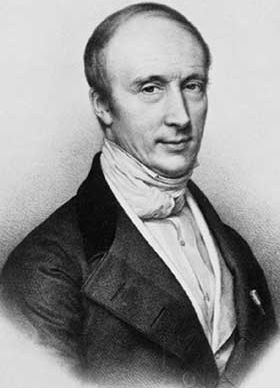
\includegraphics[height=0.4\textheight]{cauchy}
			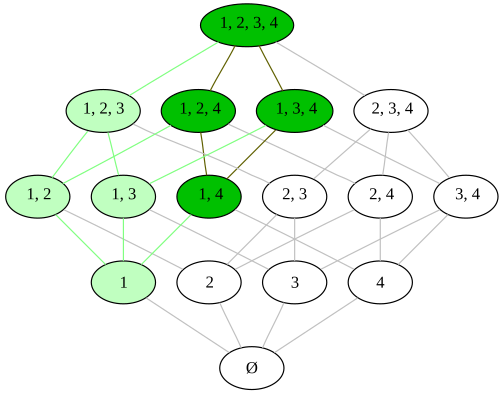
\includegraphics[height=0.4\textheight]{filter}
			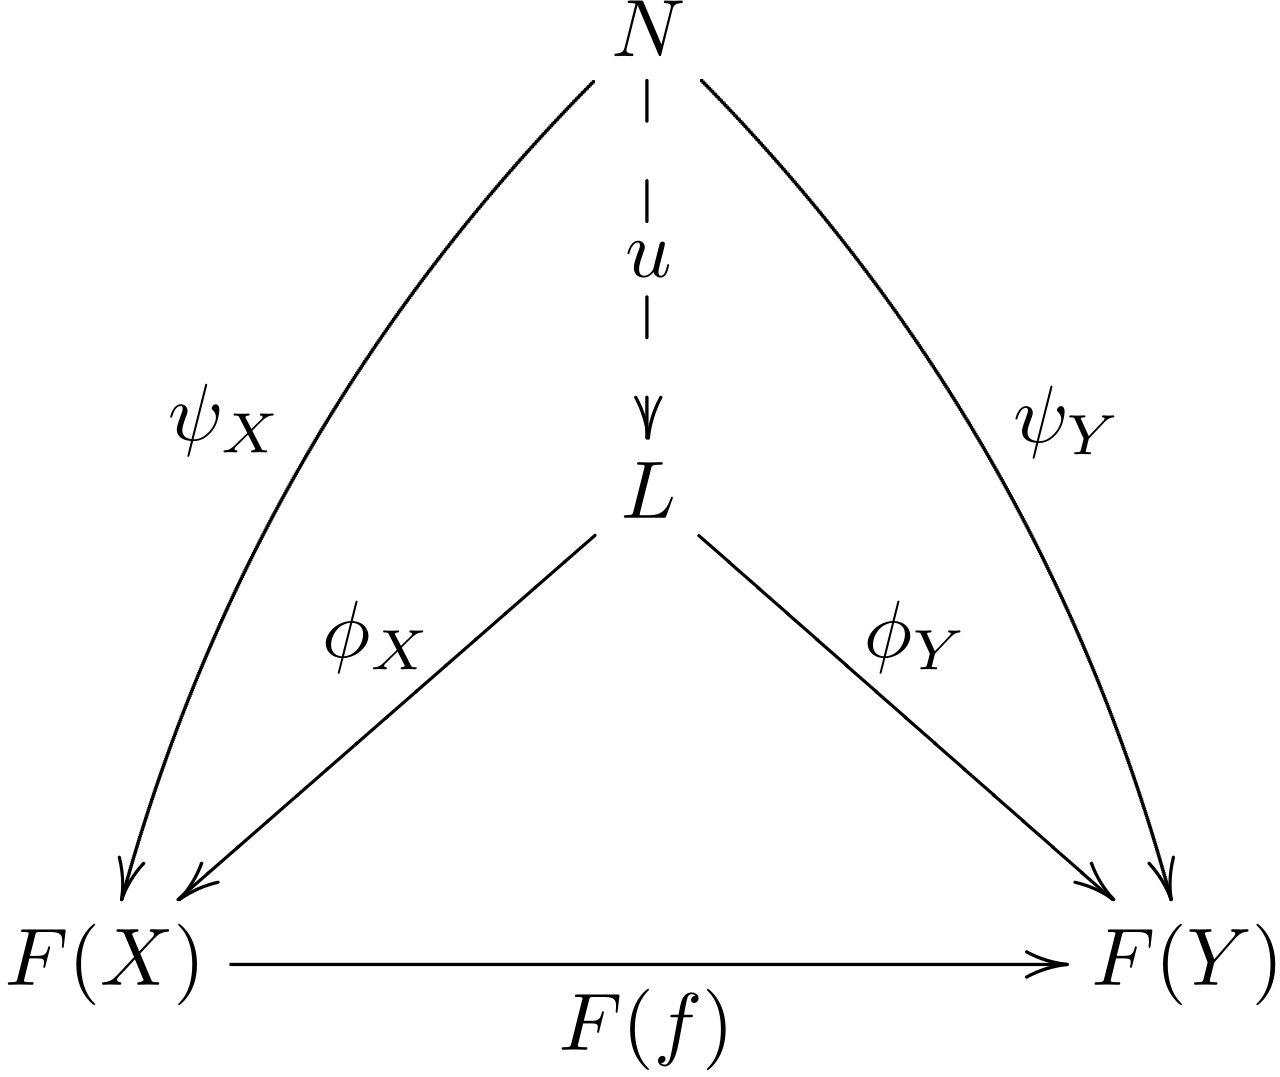
\includegraphics[height=0.4\textheight]{cone}
		\end{figure}
    \end{frame}

	\begin{frame}{Thanks}
		\centering
		{\Huge \textbf{Thank You!}}\\[2em]
		{Contact}\\[1em]
		{Email: misaka10987@outlook.com}\\
		{WeChat: misaka10987}\\
		{QQ: 2208129531}
	\end{frame}
	
\end{document}
